\begin{figure}[t]
\centering
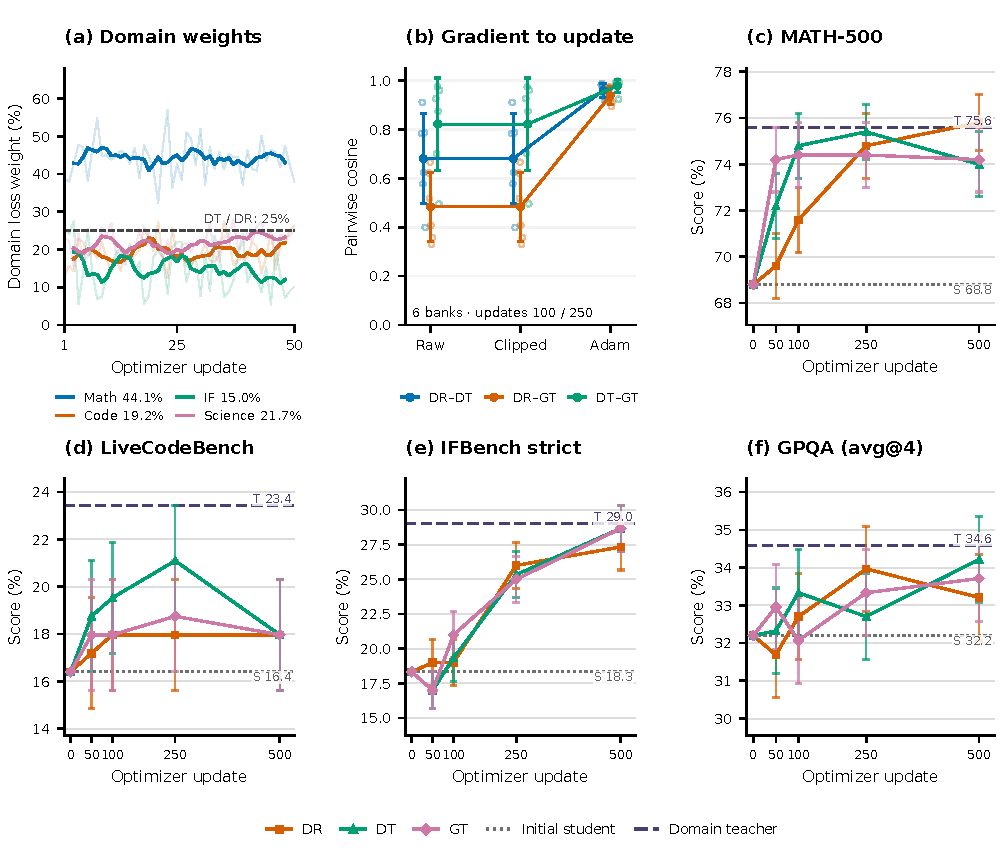
\includegraphics[width=\linewidth]{figures/nine_panel_20260914/section3_normalization.pdf}
\caption{Loss weighting, optimizer mediation, and task capability trajectories.
(a) GT domain loss weights across the first 50 updates: faint lines are individual batches, bold lines are five-batch moving averages, and legend values are arithmetic means over all 50 batches. DT and DR each fix domain weights at 25\%.
(b) Three reduction pairs before clipping, after clipping, and after a shared saved-state Adam update. Small open points are six fixed banks at updates 100/250; lines and error bars show their mean and sample standard deviation.
(c--f) GT/DT/DR scores on MATH-500, LiveCodeBench, IFBench strict, and GPQA (avg@4), with initial-student (S) and domain-teacher (T) references. Points and error bars retain the original means and sample standard deviations, computed from measured seed-42 scores and estimated seed-43/44 scores. The authors report agreement with subsequent three-seed experiments; the retained estimates are not independently verified measurements. Updates use a linear axis. Appendix Figure~\ref{fig:normalization_aggregate_support} gives the four-domain mean and worst-domain change.}
\label{fig:normalization_capability}
\end{figure}
